\documentclass[a4paper,10.5pt]{ltjsarticle}
\usepackage{graphicx}
\usepackage{caption}
\usepackage{luatexja-fontspec}
\usepackage[top=10truemm,bottom=15truemm,left=10truemm,right=10truemm]{geometry}
\usepackage{array}
\usepackage{upgreek}
\usepackage{fancyhdr}
\renewcommand{\refname}{}
\captionsetup[figure]{format=plain, labelformat=simple, labelsep=quad, font=bf}
\captionsetup[table]{format=plain, labelformat=simple, labelsep=quad, font=bf}
\parindent = 0pt
\setmainjfont[BoldFont=HiraMinProN-W6]{HiraMinPro-W3}
%[BoldFont=HGSMinchoE]{MSMincho}[BoldFont=HiraMinProN-W6]{HiraMinPro-W3}
\begin{document}

\centerline
{\huge \bfseries 調査}
\rightline
{April/29/2024}
\leftline
{}
 以下の内容は概ね2020年時点の情報で、ほぼRef\cite{1}の内容である。現状を完全に反映しているわけではない。\\
\\
\leftline{\large \bfseries 動向}\\
・2023年に中性原子の量子コンピューターが作られる(これはブレイクスルー)→量子回路はdepthが大きくなってもよくなった。また、sampling overhead は小さくしたい。\\
・中性原子としては一般にルビジウムを使う(in 2020)\\
\\
\leftline{\large \bfseries わかっていること}\\
・超伝導やシリコンスピンではできるだけ量子ビットから異質的な要素を取り除かなければならないが、中性原子ではそれらの必要がない(要調査 異質とは何か)\\
・processingする時間はとても短く、約$100\ \mathrm{\upmu s}$ 一方で、lodingとreadoutを加えると、約$200\ \mathrm{ms}$\ Ref\cite{1}→processing時間、短すぎ\\
・中性原子ではdigital processingとanalog processingができるRef\cite{1}\\
・中性原子ではレーザーを使ってgateを実現する。詳しくはpulse duration, the lazor intensity, the detuning and the phase of the laserを調整することで実現、Fidelityは99.5\%以上←これは低いとおもう。例えば、Fidelityが0.995のgateを1000個使うとしたら、その後のFidelityは$0.995^{1000}=O(10^{-3})$ Ref\cite{1}\\
・中性原子は数マイクロメートルで離れているため、相互作用をおよぼさない。しかしこれは、2000年にRydberg stateの原子がdipole-dipole interactionをすることが発見され解決されるRef\cite{1}\\
・中性原子は数マイクロメートルでも相関を持たせることができるからqubit connectivityの観点で有利→SWAP gateの使用量が減るRef\cite{1}\\
・hybrid approachではclassical computerをコスト関数の最適化に用い、quantum computerはただのサンプリングの道具\\
・Features of Anlog Quantum Simulation and Digital Quantum Simulation(in 2020)
\begin{figure}[h]
  \centering
  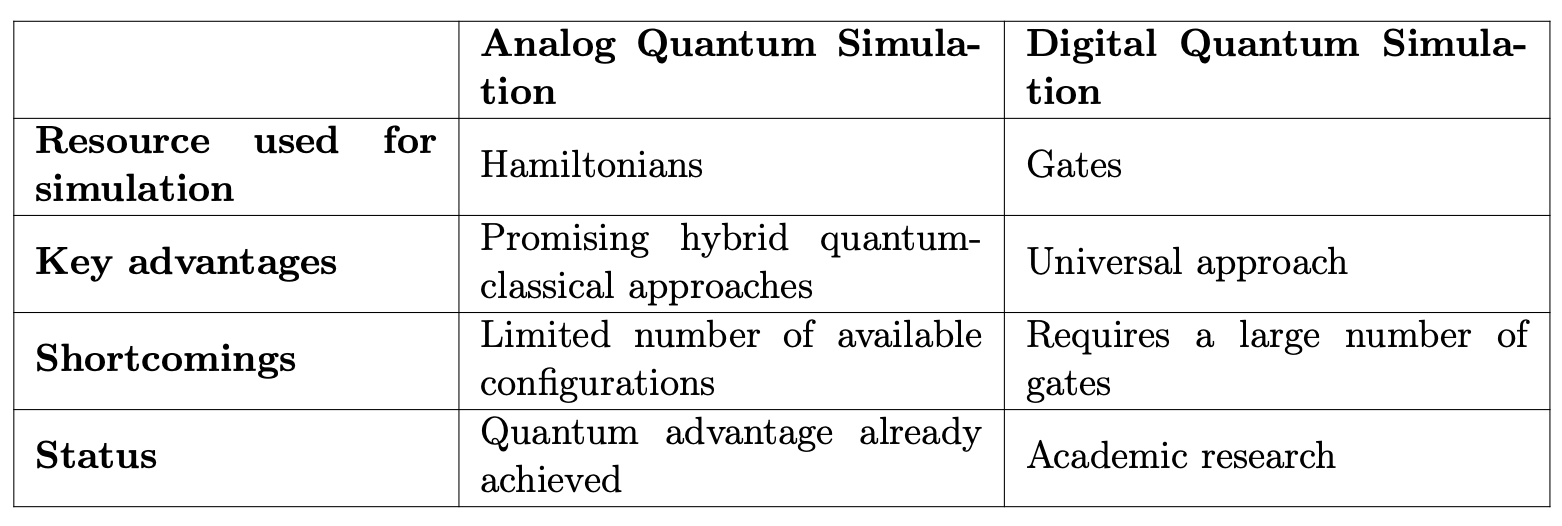
\includegraphics[scale=0.5]{figure1.png}
\end{figure}\\
・中性原子の配列をグラフ理論の点に対応させることで問題を解ける(要調査)\\
・Quantum information encoded in an incoming photon can be stored in the atomic medium using the phenomenon of electromagnetically-induced transparency(EIT). Under EIT conditions, an atomic ensemble becomes transparent to light and a single photon can propagate insaide it without losses under the form of a mixed light-matter excitation called a polariton. The polariton velocity is greatly reduced as compared to the speed of light in vacuum, and can even be tempolary set to zero Ref\cite{2}, transforming then the atomic ensenble into a quantum memory.Ref\cite{1}
\clearpage
\leftline{\large \bfseries 問題}
・FTQCは暗号に悪影響を及ぼす可能性が高い\\
・効率的なpreparationとreadoutはパフォーマンスに大きな影響を与える\\
・coherence timeで100個のgateしかできない(in 2020)Ref\cite{1}\\
・gateのFidelityは実験的に94.1\%(in 2020)Ref\cite{1}\\
・量子コンピューターではqubit同士のconnectivityが問題←中性原子はmitigate\\
・solid state platformでは新しいqubitを作るのが難しい(in 2020)\\
・parasitic charge(例えば?)によってdecoferenceが起こる\\
・analog processingのhamiltonian simulationは完全に一般化されているわけではない\\
\\
\leftline{\large \bfseries 思考}\\
・中性原子では、量子ビットを作ってからrearrangeする工程がある。これはどのようにして効率よく行われるのだろうかRef\cite{1}\\
・analog processingで行えるhamiltonian simulationの可能性はどのようなものだろうか\\
\\
{\Large \bfseries REFERENCE}
\begin{thebibliography}{1}
\vspace{-1.5cm}
  \bibitem{1} Loïc Henriet, Lucas Bequin, QUANTUM COMPUTING WITH NEUTRAL ATOMS, arXiv:2006.12326
  \bibitem{2} M. Bajcsy, A. S. Zibrov, and M. D. Lukin. Stationary pulses of light in an atomic medium. Nature, 426(6967):638–641, December 2003. DOI: 10.1038/nature02176.

\end{thebibliography}

\end{document}
